\chapter{Testing and Results} \label{chap:testing_and_results}

In order to evaluate each of the networks implemented in the previous chapter, various tests were conducted. The main forms of evaluation were previously outlines in \cref{sec:evalutaion_metrics}, allowing for a comprehensive understanding of network performance. As well as this some explanation of the findings are also given.

\section{Data Pre-processing}

The data was converted to the z-score as described in \cref{ssec:data_preprocessing_design}, which made the network learn more stably and ensure any patterns found were more robust and easily applicable to unseen data. This effect was much more apparent on the reconstructed video sequences since the intensities tended to vary much more than the intensities from integrated frames. This is since the values from the integrated frames were naturally `centred' around similar values.

\section{End-to-end Event Classification Models}

The benefits of the event driven camera (as described in \cref{ssec:event_camera_benefits}) were evident in the acquired results. \color{red} TODO: Add images of integrated frames here \color{black}. As opposed to tradition frame-based cameras, high frequency data is not lost when processing events. There are spikes for every event at a much more granular scale in the temporal dimension in the event camera when compared to the frame camera, meaning fast movements were captured more reliably since events are captured at the $\mu s$ scale, no longer restricted by the frame-rates of modern cameras (which often results in motion blur).

\subsection{Frame Integration}

It is, however, evident that modern computer vision techniques have been developed with frame-based cameras in mind, and so modern networks achieve good accuracy, and are able to find patterns well, on frame-based data. For this reason the common technique of integrating frames\cref{ssec:frame_integration} results in regular frames, akin to the ones a regular camera generates, in order to feed into such networks. It does, however, still pose many benefits when compared to the frames from a regular camera. As mentioned previously information between frames is still not lost or degraded since the events are still captured and visible in each frame. As well as this, the frames generated from events inherently focussed on the points of interest in the image, since these were the only ones in motion in the frame. Most common architectures (such as the one proposed by Raimundo F. Pinto \textit{et al.} for static hand gesture recognition\cite{StaticHandGesture}) for classical videos feature an intermediate layer to remove backgrounds and other noise from images from the image to focus on the points of interest. In this way the intermediate layer could be omitted when operating on the integrated event frames, since the output was already similar to an edge map. It is conceivable, however, that in noisy environments with lots of motion this stage would still be necessary.

It was also interesting to note the inherent ability of neuromorphic cameras to capture points of interest. When using the frame integration method, the result was very similar to an edge map, which is often the primary step of image analysis using convolutional neural networks to images in existing networks already. \Cref{fig:canny_edge_detection_nmnist} shows the effect of carrying out canny edge detection\cite{CannyEdgeDetection} on an integrated frame from the NMNIST dataset. The sample is taken from a recording of the number `0', and it can be seen that the original frame is in essence just a noisy edge map of the number. The steps taken for canny edge detection were as follows;

\begin{enumerate}
    \item Smooth image by convolving with an averaging filter of the form: $ \begin{bmatrix}
        \frac{1}{4^2} & \frac{1}{4^2}  & \frac{1}{4^2}  & \frac{1}{4^2} \\
        \frac{1}{4^2} & \frac{1}{4^2}  & \frac{1}{4^2}  & \frac{1}{4^2} \\
        \frac{1}{4^2} & \frac{1}{4^2}  & \frac{1}{4^2}  & \frac{1}{4^2} \\
        \frac{1}{4^2} & \frac{1}{4^2}  & \frac{1}{4^2}  & \frac{1}{4^2} \\
    \end{bmatrix} $
    \item Sobel edge detection was carried out in order to find the edges of the smoothed image. To do this the image was convolved with the following matrices: $ S_x =
    \begin{bmatrix}
        -1 & 0 & 1 \\
        -2 & 0 & 2 \\
        -1 & 0 & 1 \\
    \end{bmatrix} $ and $ S_y = 
    \begin{bmatrix}
        1 & 2 & 1 \\
        0 & 0 & 0 \\
        -1 & -2 & -1 \\
    \end{bmatrix} $. These matrices got the pixel gradients in the x and y directions, and taking their magnitudes ( $ \sqrt{S_x^2 + S_y^2} $ ) gives the edges map of the frame.
    \item Hysteresis thresholding allowed for weaker edges to be counted as long as they are connected to stronger ones. Then non-maximum suppression was applied to get a single line for every edge (by finding the strongest point of every line in the direction of its gradient).
\end{enumerate}

This refined edge map could have been part of the pre-processing of the data before being passed into the network, but it was found that this was not beneficial to network training. This was because some information is lost in the smoothing process, and any feature mapping was done efficiently during the training of convolutional networks anyway.

\begin{figure}[htb]%
    \centering
    \subfloat[\centering]{{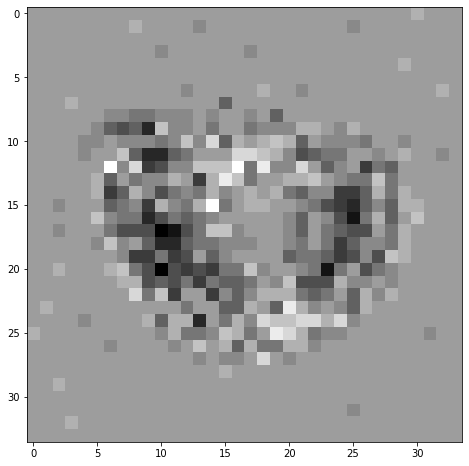
\includegraphics[width=0.18\textwidth]{testingandresults/images/denoise_origional.png}}}%
    \qquad
    \subfloat[\centering]{{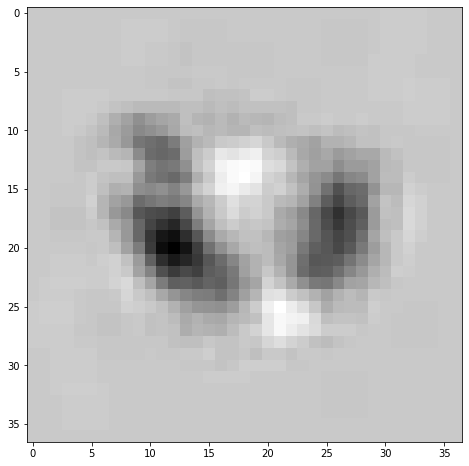
\includegraphics[width=0.18\textwidth]{testingandresults/images/denoise_smoothed.png}}}%
    \qquad
    \subfloat[\centering]{{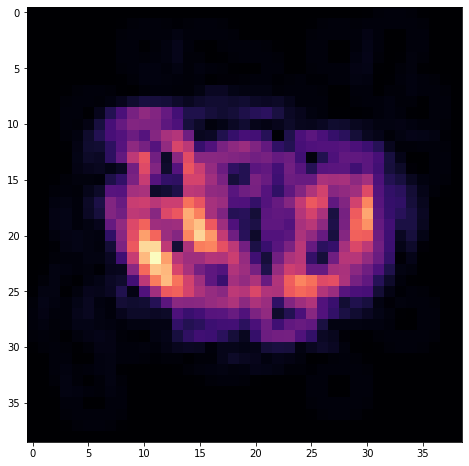
\includegraphics[width=0.18\textwidth]{testingandresults/images/denoise_edge_map.png}}}%
    \qquad
    \subfloat[\centering]{{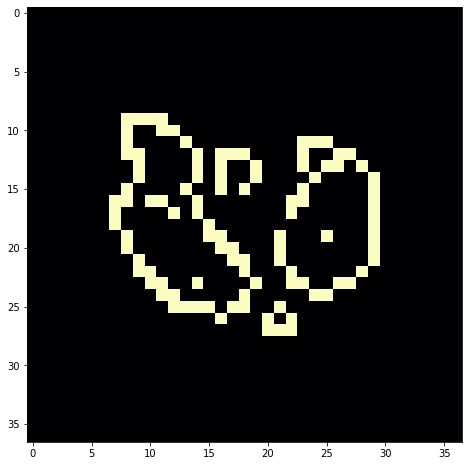
\includegraphics[width=0.18\textwidth]{testingandresults/images/denoise_hysteresis.png}}}%
    \caption{Progression of canny edge detection on integrated frame of a sample from the NMNIST dataset with class `0'. The steps are as follows; \textbf{(a)} original integrated frame, \textbf{(b)} smoothed, \textbf{(c)} edge detection, and \textbf{(d)} Non-maximum suppression and hysteresis thresholding.}%
    \label{fig:canny_edge_detection_nmnist}%
\end{figure}

\color{red} TODO: Write about the two different frame integration methods and show diagrams. \color{black}

\color{red} TODO: Write about the performance difference between synchronous and asynchronous frame integration \color{black}

\section{Two-phase Intensity Reconstruction Models}

\color{red} TODO: Write a nice intro to this section like the last section. \color{black}

\subsection{Intensity Reconstruction}

The E2VID reconstruction network (as described in \cref{ssec:video_reconstruction}) was used to recreate intensity videos from events. It was evident that the reconstructions created were robust and relatively to to life. The reconstructions were not effected by adverse lighting effects or fast motions \color{red} TODO: Add image examples \color{black}. This meant that modern computer vision techniques could still be applied to event data, while still preserving the many benefits the event model presents. It was interesting to note the performance of the reconstruction model on inputs with few moving parts. Since events are only triggered when there is an intensity change on any given pixel on the sensor, only regions with motion in them showed up as events, and the nature of all the space with no motion was not easily inferable. This can clearly be seen in \cref{fig:wave_in_lightings_reconstructions}, where only parts of the scene were accurately reconstructed. This did not, however, pose much of a problem for tasks such as gesture recognition, since the motion is exactly what is being classified, however for other tasks such as object recognition it had to be ensured that there was some sort of motion of either the object or the camera for the reconstruction algorithm to be effective.

\color{red} TODO: Include image and explanations of NMNIST reconstructions \color{black}

\Cref{fig:wave_in_lightings_reconstructions} shows that event-cameras do indeed allow for higher fidelity video capture in a wider range of lighting conditions that frame-based cameras (as explained in \cref{ssec:event_camera_benefits}). In all lighting conditions the video reconstruction was largely the same, since the events triggered were very similar in all cases. The logarithmic characteristics of the event-sensor pixels are the reason for this, since the thresholds for the triggering of events is not static. Since the reconstructions are consistent across lighting conditions, this also means that the reconstruction is more reliable, and the classification algorithm works better in adverse conditions in general \color{red} TODO: get figures and images to prove this \color{black}.

\begin{figure}[htb]%
    \centering
    \subfloat[\centering]{{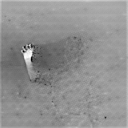
\includegraphics[width=0.18\textwidth]{testingandresults/images/dvs_wave_fluorescent_led.png}}}%
    \qquad
    \subfloat[\centering]{{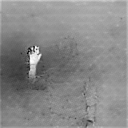
\includegraphics[width=0.18\textwidth]{testingandresults/images/dvs_wave_fluorescent.png}}}%
    \qquad
    \subfloat[\centering]{{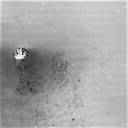
\includegraphics[width=0.18\textwidth]{testingandresults/images/dvs_wave_lab.png}}}%
    \qquad
    \subfloat[\centering]{{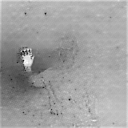
\includegraphics[width=0.18\textwidth]{testingandresults/images/dvs_wave_led.png}}}%
    \qquad
    \subfloat[\centering]{{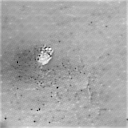
\includegraphics[width=0.18\textwidth]{testingandresults/images/dvs_wave_natural.png}}}%
    \caption{A waving motion being reconstructed from events captures by DVS128 event camera under different lighting conditions.The lighting conditions are as follows; \textbf{(a)} fluorescent led, \textbf{(b)} fluorescent, \textbf{(c)} lab lighting, \textbf{(d)} led lighting and \textbf{(e)} natural lighting.}%
    \label{fig:wave_in_lightings_reconstructions}%
\end{figure}

\subsection{Classification Results}

\subsubsection{NMNIST Dataset}

The confusion matrices for the classification of the frame-integrated  NMNIST dataset can be seen in \cref{fig:nmnist_c_matrices}. In terms of precision of classification, all networks perform relatively well. However, the 3D convolutional network and the custom convolutional LSTM network were marginally more effective, achieving a higher accuracy and correctly classifying more challenging event streams. Where this is most apparent is when classifying numbers such as 3, since with the base convolutional LSTM network these were sometime misclassified as an 8 or 9.

The confusion matrices for the classification of the intensity reconstructed NMNIST dataset can be seen in \cref{fig:nmnist_recon_c_matrices}. \color{red} TODO: Write more about this. \color{black}

The drawback to the 3D convolutional network is that the number of trainiable parameters (as can be seen in \cref{ssec:conv_3d_network_design}) is much higher than the other networks, and so the training and inference times were considerably higher than the other networks as well (as can be seen in \cref{tab:network_training_times}).

\begin{figure}[htb]%
    \centering
    \subfloat[\centering]{{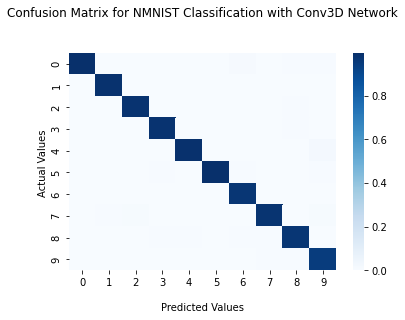
\includegraphics[width=0.4\textwidth]{testingandresults/images/c_matrix_nmnist_conv3d.png}}}%
    \qquad
    \subfloat[\centering]{{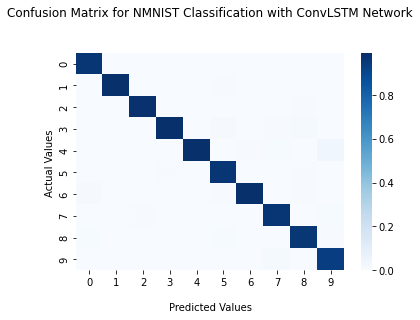
\includegraphics[width=0.4\textwidth]{testingandresults/images/c_matrix_nmnist_convlstm.png}}}%
    \qquad
    \subfloat[\centering]{{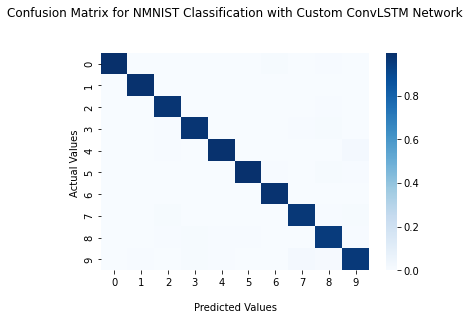
\includegraphics[width=0.4\textwidth]{testingandresults/images/c_matrix_nmnist_custom_convlstm.png}}}%
    \caption{Confusion matrices for frame-integrated NMNIST classification with various networks; \textbf{(a)} conv3D, \textbf{(b)} convLSTM, \textbf{(c)} custom convLSTM.}%
    \label{fig:nmnist_c_matrices}%
\end{figure}

\begin{figure}[htb]%
    \centering
    \subfloat[\centering]{{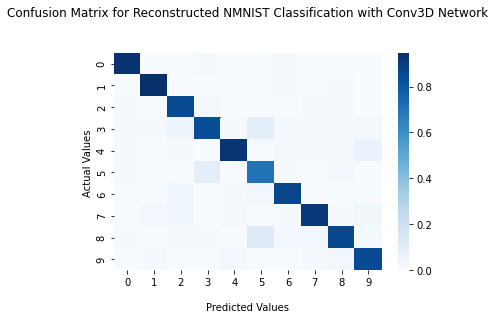
\includegraphics[width=0.4\textwidth]{testingandresults/images/c_matrix_nmnist_recon_conv3d.png}}}%
    \qquad
    \subfloat[\centering]{{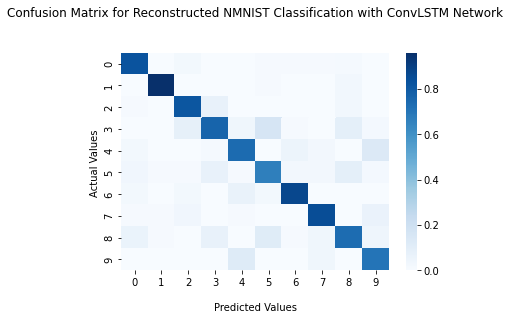
\includegraphics[width=0.4\textwidth]{testingandresults/images/c_matrix_nmnist_recon_convlstm.png}}}%
    \qquad
    \subfloat[\centering]{{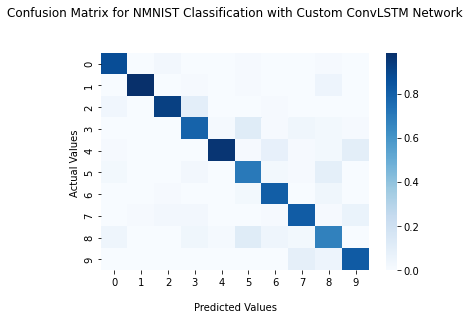
\includegraphics[width=0.4\textwidth]{testingandresults/images/c_matrix_nmnist_recon_custom_convlstm.png}}}%
    \caption{Confusion matrices for intensity reconstructed NMNIST classification with various networks; \textbf{(a)} conv3D, \textbf{(b)} convLSTM, \textbf{(c)} custom convLSTM.}%
    \label{fig:nmnist_recon_c_matrices}%
\end{figure}

\Cref{tab:conv3d_nmnist_evaluation_metrics}, \cref{tab:conv_lstm_nmnist_evaluation_metrics}, and \cref{tab:custom_conv_lstm_nmnist_evaluation_metrics} show the performance evaluation of each of the networks on the frame-integrated NMNIST dataset in more detail.

\Cref{tab:conv3d_nmnist_recon_evaluation_metrics}, \cref{tab:conv_lstm_nmnist_recon_evaluation_metrics}, and \cref{tab:custom_conv_lstm_nmnist_recon_evaluation_metrics} show the performance evaluation of each of the networks on the intensity reconstructed NMNIST dataset in more detail.

\color{red} TODO: Write more about the meaning of the tables. \color{black}

\color{red} TODO: Make more custom convolution LSTMs \color{black}

\subsubsection{DVS128 Gesture Dataset}

The confusion matrices for the classification of the frame-integrated DVS128 Gesture dataset can be seen in \cref{fig:dvs128_c_matrices}. The variance in performance between the networks is more apparent in this dataset than for the NMNIST dataset. The reason for this is that not only is object detection (of the human body) being undertaken by the system, but also action recognition across frames. It is evident that actions 4 and 5 (right arm clockwise and right arm counter-clockwise), as well as actions 6 and 7 (left arm clockwise and left arm counter-clockwise), were often misclassified as one another. The reason for this was that with length 20 frame integrated videos the fast rotational movement results in frames that look very similar in both directions. \color{red} TODO: Maybe try to get some pictures to prove this. \color{black} Other mistakes were more often made with the 3D convolutional network. For example 10 (air guitar) was quite often predicted for cases of classes 8 and 9 (air roll and air drums). 

The confusion matrices for the classification of the intensity reconstructed DVS128 Gesture dataset can be seen in \cref{fig:dvs128_recon_c_matrices}. \color{red} TODO: Write more about this. \color{black}

\begin{figure}[htb]%
    \centering
    \subfloat[\centering]{{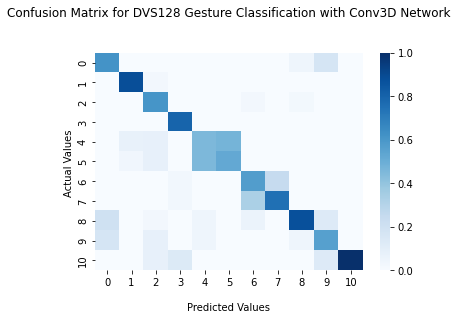
\includegraphics[width=0.4\textwidth]{testingandresults/images/c_matrix_dvs128_conv3d.png}}}%
    \qquad
    \subfloat[\centering]{{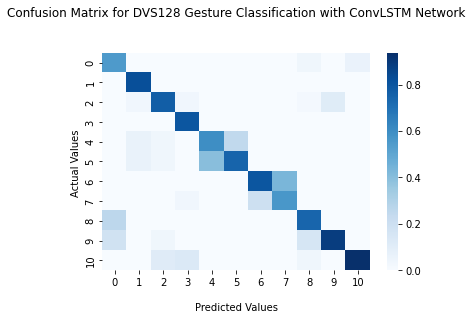
\includegraphics[width=0.4\textwidth]{testingandresults/images/c_matrix_dvs128_convlstm.png}}}%
    \qquad
    \subfloat[\centering]{{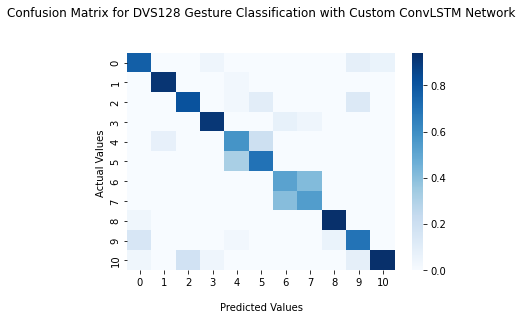
\includegraphics[width=0.4\textwidth]{testingandresults/images/c_matrix_dvs128_custom_convlstm.png}}}%
    \caption{Confusion matrices for frame-integrated  DVS128 Gesure classification with various networks; \textbf{(a)} conv3D, \textbf{(b)} convLSTM, \textbf{(c)} custom convLSTM.}%
    \label{fig:dvs128_c_matrices}%
\end{figure}

\begin{figure}[htb]%
    \centering
    \subfloat[\centering]{{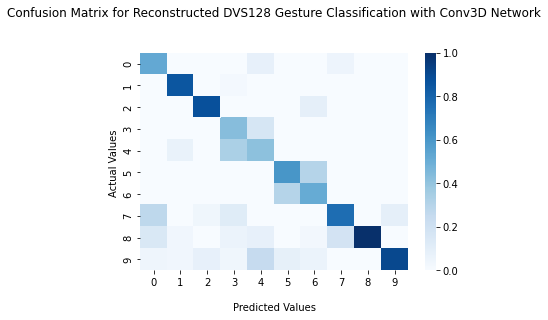
\includegraphics[width=0.4\textwidth]{testingandresults/images/c_matrix_dvs128_recon_conv3d.png}}}%
    \qquad
    \subfloat[\centering]{{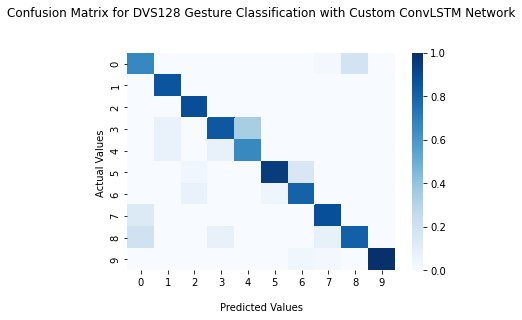
\includegraphics[width=0.4\textwidth]{testingandresults/images/c_matrix_dvs128_recon_custom_convlstm.png}}}%
    \caption{Confusion matrices for frame-integrated  DVS128 Gesure classification with various networks; \textbf{(a)} conv3D, \textbf{(b)} custom convLSTM.}%
    \label{fig:dvs128_recon_c_matrices}%
\end{figure}

\Cref{tab:conv3d_dvs128_evaluation_metrics}, \cref{tab:conv_lstm_dvs128_evaluation_metrics}, and \cref{tab:custom_conv_lstm_dvs128_evaluation_metrics} show the performance evaluation of each of the networks on the frame-integrated DVS128 Gesture dataset in more detail.

\Cref{tab:conv3d_dvs128_recon_evaluation_metrics} and \cref{tab:custom_conv_lstm_dvs128_recon_evaluation_metrics} show the performance evaluation of each of the networks on the intensity reconstructed DVS128 Gesture dataset in more detail. 
\color {red} TODO: Write about how frame integration is a more compact information store since the convLSTM couldn't even run for DVS128 reconstructions. \color{black}
\color{red} TODO: Write more about the meaning of the tables. \color{black}
\color{red} TODO: Make more custom convolution LSTMs \color{black}

\subsection{Network Comparisons}

\begin{table}[htb]
    \centering
    \begin{tabular}{|| c | c | c ||}
        \hline
        Network     & NMNIST & DVS128 Gesture \\
        \hline \hline
        Conv3D Event Classifier          & 98.22\%   &   69.44\%    \\
        \hline
        Conv2D LTSM Event Classifier         & 97.48\%   &    71.53\%    \\
        \hline
        Custom LTSM Event Classifier         & 97.88\%  &   76.39\%     \\
        \hline
        Conv3D Reconstruction Classifier           & 86.67\%    &   63.26\%    \\
        \hline
        Conv2D LTSM Reconstruction Classifier          & 79.60\%   &  -    \\
        \hline
        Custom LTSM Reconstruction Classifier         & 83.20\%  &   82.95\%   \\
        \hline
    \end{tabular}
    \caption{A table showing classification accuracies of various models.}
    \label{tab:network_performances}
\end{table}

The full table of classification accuracies can be seen in \cref{tab:network_performances}. Here, the different strengths of the various networks becomes apparent in this comparison. For the simple object classification task on the NMNIST dataset, the higher capacity 3D convolutional network outperformed the others. However, in the more complex task of gesture recognition on the DVS128 Gesture dataset it struggled. The reason for this is that though it is excellent at detecting spacial patterns in each frame, it is less able to detect the temporal patterns prevalent in the gestures.

\begin{table}[htb]
    \centering
    \begin{tabular}{|| c | c | c ||}
        \hline
        Network     & NMNIST & DVS128 Gesture \\
        \hline \hline
        Conv3D Event Classifier          & 1h43m03s   &   0h34m49s    \\
        \hline
        Conv2D LTSM Event Classifier         & 1h03m09s   &    0h08m33s    \\
        \hline
        Custom LTSM Event Classifier         &  1h12m10s  &    \color{red} 1h24m19s \color{black}    \\
        \hline
        Conv3D Reconstruction Classifier        &  0h05m02s    &    1h09m43s  \\
        \hline
        Conv2D LTSM Reconstruction Classifier        &  0h14m28s    &      \\
        \hline
        Custom Conv2D LTSM Reconstruction Classifier         &  0h03m26s \color{red} why so short \color{black}  &    3h13m45s   \\
        \hline
    \end{tabular}
    \caption{A table showing training times various models.}
    \label{tab:network_training_times}
\end{table}


The training times for each of the networks on the datasets can be seen in \cref{tab:network_training_times}. It is evident that the networks with a higher capacity had higher training times. The 3D convolution network in particular had much longer training times than the other two networks, since it had many more parameters to optimise via back-propagation. It should be noted that for the networks in \color{red} red \color{black} the system encountered an Out Of Memory (OOM) error when attempting create a tensor of larger batch size. For these cases a smaller batch size was used, resulting in slightly higher training times, as well as possible skewed results.